% use the answers clause to get answers to print; otherwise leave it out.
\documentclass[12pts,answers]{exam}
\RequirePackage{amssymb, amsfonts, amsmath, latexsym, verbatim, xspace, setspace}
\usepackage{graphicx}

% By default LaTeX uses large margins.  This doesn't work well on exams; problems
% end up in the "middle" of the page, reducing the amount of space for students
% to work on them.
\usepackage[margin=1in]{geometry}
\usepackage{enumerate}
\usepackage[hidelinks]{hyperref}

% Here's where you edit the Class, Exam, Date, etc.
\newcommand{\class}{NPRE 498}
\newcommand{\term}{Fall 2018}
\newcommand{\assignment}{Final}
\newcommand{\duedate}{2018.12.12}
%\newcommand{\timelimit}{50 Minutes}

\newcommand{\nth}{n\ensuremath{^{\text{th}}} }
\newcommand{\ve}[1]{\ensuremath{\mathbf{#1}}}
\newcommand{\Macro}{\ensuremath{\Sigma}}
\newcommand{\vOmega}{\ensuremath{\hat{\Omega}}}

% For an exam, single spacing is most appropriate
%\singlespacing
\onehalfspacing
% \doublespacing

% For an exam, we generally want to turn off paragraph indentation
\parindent 0ex

%\unframedsolutions

\begin{document} 

% These commands set up the running header on the top of the exam pages
\pagestyle{head}
\firstpageheader{}{}{}
\runningheader{\class}{\assignment\ - Page \thepage\ of \numpages}{Due \duedate}
\runningheadrule

\class \hfill \term \\
\assignment \hfill Due \duedate\\
\rule[1ex]{\textwidth}{.1pt}
%\hrulefill

\section{Introduction}
Pyroprocessing is an electrochemical separation method used primarily for metallic fast reactor fuel.
This reprocessing technique uses molten salt, which differs depending on the facility, to provide a medium for current to travel across.
Molten salt such as LiCl-KCl has a broader stability range comparative to water, allowing high potentials to be used for separation.
Traditionally, separation would be conducted in a nitric acid which uses water as its medium.
Water, however, has a significantly lower stability compared to molten salt.
This becomes a problem when considering higher elements such as lanthanides and actinides.
Controlling the oxidation states of these elements often requires potentials outside the stability of water.
Hence, Pyroprocessing was born to improve nonproliferation and reprocessing capabilities.
\\ \\
In addition to the additional redox control of higher elements, we also co-extract materials of interest such that they cannot easily be refined for weapons.
This is done through the electrorefining and electrowinning stages by separating a pure Uranium stream as well as a Uranium/Transuranic mix stream. 
The U/TRU can then be readily used for fuel fabrication while maintaining proliferation resistance.
Although the facility is great in terms of safeguards, pyroprocessing has its share of drawbacks as well.
Currently, pyroprocessing can only be performed as a batch process, which signficantly limits throughput compared to a continuous facility. 
Additionally, the safety and economical concerns of running a molten salt plant are much greater than a nitric acid one.
Despite these downsides, pyroprocessing is an efficient use of electrochemical separation and leader in proliferation resistant separations.

\section{Theory and Mechanisms}
\subsection{Electrochemical Separations}
Electrochemical separation is the driving force behind pyroprocessing. Electrochemistry relies on the use of Gibbs free energy to determine the required amount of energy to drive a reaction forward.

\begin{figure}[h]
	\centering
	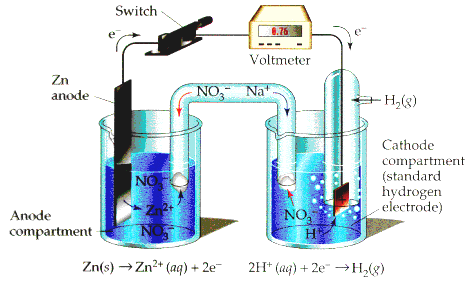
\includegraphics[width=0.8\linewidth]{electrochem}
	\caption{Basic example of movement of ion within galvanic cell \cite{angel}.}
\end{figure}

Figure 1 demonstrates an electrochemical process that generates electricity as a basic example.
The processes described here follow the same principles, however, require energy to run.
In both cases, ions are exchanged between the anode and cathode in an attempt to balance the potential difference.
In the case of pyroprocessing, the potential difference is artificially applied.
A number of different anodes and cathodes are used to force the desired ions to deliver charge from one end of the cell to the other.
These ions that collect on the surface of the cathode can then be removed from the liquid and separated from the rest of the solution.
By controlling the voltage of the solution as well as the composition of the anode, cathode, and electrolyte we can ensure the removal of unwanted elements/isotopes.

\section{Process}
There are multiple different designs for a pyroprocessing facility, the most prominent being from ANL, INL, and KAERI. In order to encompass them all, we must take a generic approach. This is accomplished by including the following sub-processes: Voloxidation, Electroreduction, Electrorefining, and Electrowinning. While Electrorefining is the process of primary concern, each of the processes has an important in role in various processing plants. Figure 2 shows the flowsheet of a pyroprocessing plant capable of separating MOX fuel as well as fast reactor molten salt fuel.
\begin{figure}[h]
	\centering
	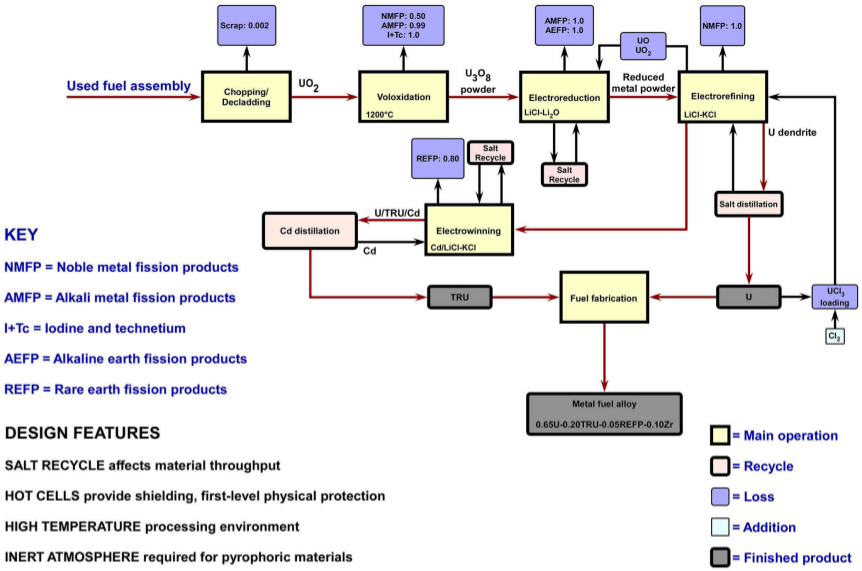
\includegraphics[width=0.9\linewidth]{borrelli_flowsheet.png} 
	\caption{Flow diagram of generic Pyroprocessing plant \cite{borrelli_approaches_2017}.}
\end{figure}


\subsection{Voloxidation}
Voloxidation is used following the chopping and decladding of the spent fuel. The process is very similar to annealing in regards to materials. The Uranium dioxide is heated to temperatures around 700-1000$^\circ C$ which allows gases and some fission products to escape the fuel pellet. UO$_2$ is converted to U$_3$O$_8$ in this process as well\cite{organisation}. Voloxidation, in most cases, takes place in air which provides plenty of oxygen for oxidization of solid UO$_2$ \cite{jubin_spent_2009}:

\[ 3UO_2 + O_2 \rightarrow U_3O_8 \]

The above reaction is possible because of the expansion of uranium at elevated temperatures. A positive feedback is also established as the Uranium dioxide converts to yellowcake powder, the fuel element expands exposing more Uranium dioxide to oxygen. The rate of this reaction/conversion is dependent on the temperature and gas used. Higher temperatures will yield a faster reaction rate, however, even ~500 $^\circ C$ is sufficient for 99\% reduction in 4 hours.

An added benefit of running a pyroprocessing voloxidation sub-process at the temperatures previously mentioned, 700-1000$^\circ C$, is the removal of some fission products. The PRIDE facility at KAERI takes it a step further and voloxidates at 1250$^\circ C$ to remove troublesome fission products at the beginning of the cycle\cite{organisation}:

\[ 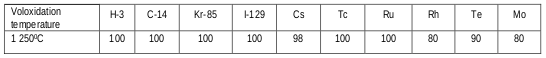
\includegraphics[width=\linewidth]{volox_table.png} \]

As shown in the table above, a majority of high activity isotopes are removed from the system at the beginning of pyroprocessing. This protects equipment and workers down the line. These gases are sent to the off-gas treatment facility that makes use of various scrubbing techniques such as liquid scrubbing, cyrogenic distillation (for the krypton), caustic scrubbing, etc \cite{jubin_spent_2009}.

\begin{figure}[h]
	\centering
	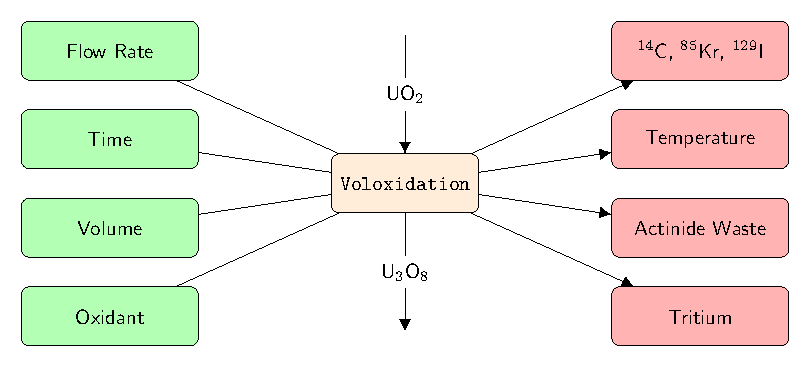
\includegraphics[width=0.7\linewidth]{volox}
	\caption{Enlarged mass balance area of Voloxidation \cite{westphal_pyre_2018}.}
\end{figure}

The above flowchart is a closer look on the dependencies and outputs of the voloxidation process. The green blocks contain parameters that affect efficiency and reaction rate while the red boxes indicate wastes or observable outputs (temperature is both an input and observable quantity). The yellowcake from voloxidation is then sent to become a molten salt for use in the electrorefiner.

\subsection{Electroreduction}
Following off-gassing and conversion to yellowcake, the non-metallic fuel must be converted and reduced to molten salt mixture. Most cases this is done with a LiCl-KCl salt eutectic combined with Li$_2$O catalyst. The electrolytic reduction phase consists of three main parts: UO$_2$ recovery, reduction, and RE removal.

\begin{figure}[h]
	\centering
	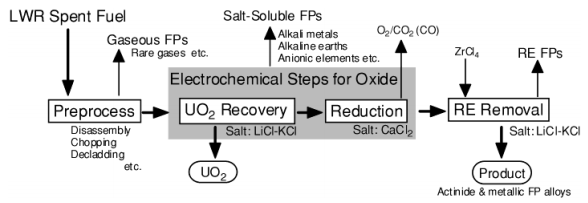
\includegraphics[width=\linewidth]{reduction_flow}
	\caption{Electroreduction flow sheet \cite{ohta}.}
\end{figure}

First step in electrolytic reduction is the recovery of UO$_2$ before reducing the remaining material.
The following equations dictate the transfer of Uranium from the anode to the cathode.

\[ UO_2 \rightarrow UO_2^{2+}(LiCl-KCl) + 2e^{2-} \hspace{6mm} anode \]
\[ UO^{2+}(LiCl-KCl) + 2e^{2-} \rightarrow UO_2 \hspace{6mm} cathode \]

As in other separations technologies, noble metals can often follow the uranium through the rest of the process.
The lurking noble metal fission products cause an increase in radioactivity of the UO$_2$ stream. 
Therefore, the weight percent dissolution of Uranium is critical in reducing the amount of waste that follows to the product stream.
Lithium Oxide can also be used as a catalyst to draw Uranium to the cathode while leaving the noble metal fission products in the salt.
This is done with 1-3wt\% Li$_2$O in the following equations \cite{hur_electrochemical_nodate}:

\[ Li_2O \rightarrow 2Li^+ + O^{2-} \]
\[ UO_{x/2} + xLi \rightarrow U + xLi_2O \]

These equations make a continuously driven loop dragging Uranium (either UO$_2$ or U$_3$O$_8$) from the anode to the cathode. 
Disproportionated Lithium ions from the first equation break apart the Uranium and Oxide, with help from the electric potential.
The U will collect on the cathode while the Li$_2$O is recycled and drives the first equation to the right again. 
Reduction then occurs on the cathode where the U, TRU, rare earths and noble metals have collected.
This is achieved by evolving oxygen gas along the anode using the following reactions\cite{hur_electrochemical_nodate,organisation}:

\[ Li^+ \rightarrow Li + e^- \hspace{10mm} Cathode \]
\[ M_xO_y + 2yLi \rightarrow xM + yLi_2O \hspace{10mm} Cathode \]
\[ O^{2-} \rightarrow 0.5O_2 + 2e^- \hspace{10mm} Anode \]

Electrochemical reduction results in an alloy of reduced U/TRU/RE/NM, however, we want to minimize the amount of RE and NM in the product.
We've touched already on how to reduce the quantity of NM and for the final step the RE must be removed.
The RE FPs can be removed from the alloy by substituting another chloride into the LiCl-KCl eutectic.
In the case of Ohta et al. ZrCl$_4$ was considered \cite{ohta}:

\[ 3ZrCl_4(LiCl-KCl + RE \rightarrow 3Zr + 4RECl_3(LiCl-KCl) \]

This process is shown to have a decontamination factor of 10 in regards to separating REs from actinides \cite{sakamura}. Additionally, by using Zirconium as the metal substitute, it is compatible with fuel fabrication later \cite{ohta}.
\subsection{Electrorefining}
Electrorefining is the primary process in pyroprocessing, and is the feed point for fast reactor fuel, since it does not require reduction or chopping.
Being the most important process, it is also the most complex with a multitude of input parameters and outputs. 
The goal of the refining process is to separate the Uranium and TRU from the alloy ingot formed in the reduction phase.
Two streams will be formed for the fabrication of fuel. One stream that is a mix of U/TRU at the desired ratio, and the other a pure stream of Uranium.
The refining step's efficiency relies on temperature and current primarily, however, advanced methods are being developed.
KAERI for example has conducted work on adding a central stirrer, vacuum pressure, and rotating the anode \cite{lee_advanced}.
The rotation aims to mix the Uranium in the salt such that none gets stuck on the bottom or edges of the vessel. 
Stirring too vigorously, however, can lead to the removal of uranium dendrites from the cathode thereby decreasing efficiency.\\

\begin{figure}[h]
	\centering
	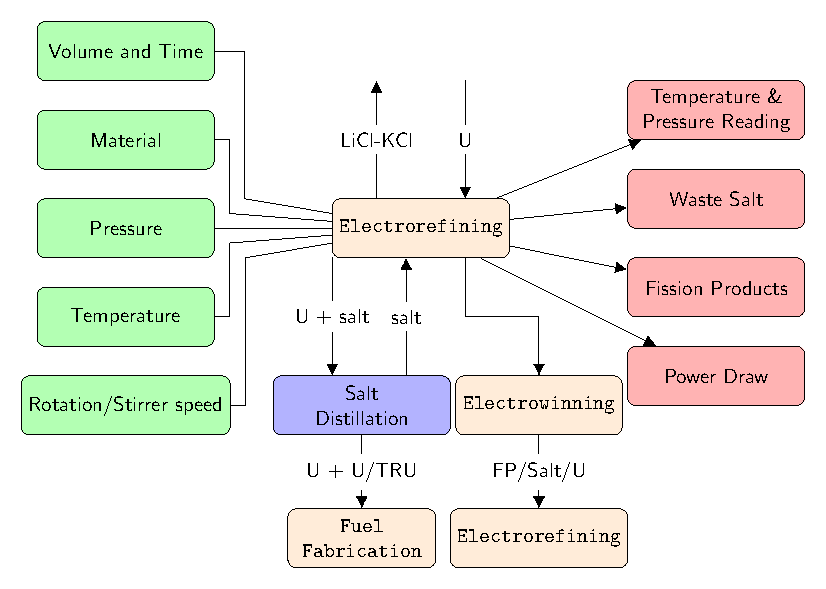
\includegraphics[width=0.8\linewidth]{refining}
	\caption{Enlarged mass balance area of Electrorefining \cite{westphal_pyre_2018}.}
\end{figure}

Figure 5 shows the final removal of fission products, RE, and contaminated salt. 
The governing reactions that allow this process to work are based on the stability constants and oxidization potential of the remaining fission products.
The voltage used is such that Uranium is unstable in the chloride form, 0.5~1V \cite{organisation}, while transuranics have a higher stability. 
This leads to TRU remaining in chloride form, along with some Uranium, and pure Uranium accumulating on the cathode.
The chloride reaction follows the below equation, and will run to the right as long as there is Uranium within the salt \cite{organisation}.

\[ UCl_3+TRU(RE) \rightarrow U + TRU(RE)Cl_3 \]
\[ UCl_3 + 3Na \rightarrow 3NaCl + U \]
\[ UCl_3 + 3Cs \rightarrow 3CsCl + U \]
\[ UCl_3 + Pu \rightarrow PuCl_3 + U \hspace{10mm} \delta G = -22.44kcal \]
\[ 4UCl_3 + 3Zr \rightarrow 3ZrCl_4 + 5U \hspace{10mm} \delta G = 31.123kcal \]

As shown by the reactions above, the TRU have a favorable gibbs free energy value for spontaneous reaction while the transition metals do not \cite{supy}.
This leads to the transition metals remaining in anode basket while the TRU are drawn into the liquid cadmium cathode \cite{lee_korean_2011}.


\subsection{Electrowinning}
The Electrorefiner accumulates TRUs and rare earth fission products within the salt.
These isotopes build up and require separation and disposal, therefore the salt from the refiner is sent to the electrowinner.
This stage further purifies the salt by targeting the electric potential of TRUs, RE and Uranium again \cite{lee_korean_2011,organisation}.
Placed in liquid cadmium once again, the three groups have overlapping electric potentials.
Therefore, the three groups will all deposit in the cadmium \cite{lee_korean_2011}. 
While the refiner's role is to generate a stream of pure Uranium, the electrowinner performs co-extraction of Uranium and TRUs.
This inherit proliferation resistance is a main draw of the pyroprocessing technique.
Rare earths are still present on the cadmium therefore further separations must be conducted.
These elements are removed through the addition of CdCl$_2$ which oxidizes the rare earths while the uranium and TRUs are unaffected.
These oxidized elements fall back into the salt, leaving the purified U/TRU stream on the electrowinner.

\begin{figure}[h]
	\centering
	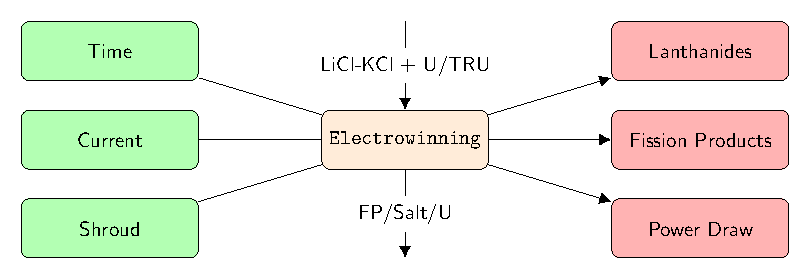
\includegraphics[width=0.7\linewidth]{winning}
	\caption{Enlarged mass balance area of Electrowinning \cite{westphal_pyre_2018}.}
\end{figure}

Figure 6 shows the elements separated and used for observation. The use of a porous shroud has been suggested on the anode to increase surface area while limiting Cl$_2$ gas production from the LiCl-KCl eutectic. Such an addition has been theorized to improve separation efficiency and protecting against corrosion \cite{kim_development_2013}.

\section{Summary}
Pyroprocessing is a batch electrochemical separations process for the co-extraction of Uranium and Transuranics.
The facility takes advantage of the f-orbital elements' close electric potentials in certain media to perform this co-extraction. 
With the use of the additional voloxidation and electroreduction sub-processes, pyroprocessing is able to refine lwr spent fuel as well as metallic fast reactor fuel.
The voloxidation stage handles the release of noble gases and troublesome fission products such as carbon-14, krypton and iodine if run at high enough temperature.
This separates a bulk of the radioactivity at the beginning of the batch, sparing unnecessary damage to instrumentation or workers.
The reduction step takes the powder from voloxidation and reduces the uranium, transuranics, noble metal fission products and rare earth fission products.
The use of a Li$_2$O catalyst in addition to the LiCl-KCl eutectic provides an expedited route for Uranium to deposit on the cathode, resulting in an ingot consisting of U/TRU/RE/NM. \\ \\
After the reduction stage, the light water reactor spent fuel can now enter the refiner just as metallic fast reactor spent fuel does.
Electrorefiners are responsible for the first product stream of the batch.
The process takes place inside the LiCl-KCl eutectic with a graphite cathode for an output stream of pure Uranium. 
Taking advantage of the stability constants of TRU chloride compounds compared to Uranium.
TRUs are substantially more stable in their chloride form than Uranium, leading to Uranium being drawn out of the salt first.
Additionally, noble metals lack the gibbs free energy to be reduced and enter the salt to begin with.
This leaves noble metals in the anode basket, TRU and RE in the LiCl-KCl eutectic, and Uranium accumulating on the graphite cathode.
Finally the salt containing TRU and RE is sent to the electrowinning stage for final separations. 
The Electrowinning process is similar to the refiner, however, focuses on the co-extraction of Uranium and TRUs.
Again, the similarity in electrochemical potential is used to collect essentially all of the Uranium, TRU, and RE on a liquid cadmium cathode.
Following this, a CdCl$-_2$ oxidant is used to oxidize the rare earth elements on the cathode which proceed to fall back into the molten salt.
This process leaves a stream of co-extracted Uranium and TRU for fabricating fast reactor fuel, and extremely proliferation resistant. \\ \\

The versatility, effectiveness and safety of pyroprocessing plants has been demonstrated through a detailed analyses of the chemistry behind each main process. 
Electrochemical separation of heavy elements such as U and TRU are not viable in water based solutions such as nitric acid because of water's own stability constant.
The addition of a molten salt eutectic allows a potential strong enough for direct separation of key isotopes and element groups for fuel fabrication. 
Combining with other known separations techniques like voloxidation, off-gas treatment and salt distillation, a majority of undesirable elements are separated from the waste salt as well.

\bibliographystyle{ieeetr}
\bibliography{bibliography}
\end{document}